\documentclass[aps,prx,reprint,superscriptaddress,nofootinbib,longbibliography]{revtex4-2}

\usepackage{amsmath,amssymb,bm,mathtools}
\usepackage{graphicx}
\usepackage{booktabs}
\usepackage{microtype}
\usepackage{hyperref}
\usepackage{xcolor}
\usepackage{siunitx}
\usepackage{amsthm}

\hypersetup{colorlinks=true,linkcolor=black,citecolor=black,urlcolor=blue}
\graphicspath{{figures/}}
\newtheorem{theorem}{Theorem}
\newtheorem{corollary}{Corollary}
\newcommand{\Tr}{\operatorname{Tr}}
\newcommand{\deff}{d_{\rm eff}}

\begin{document}

\title{Measurement-Accessible Quantum Tangent Geometry: Rank Typicality Without Isotropy}

\author{Marwan Ait Haddou}
\thanks{ORCID: \href{https://orcid.org/0009-0008-1734-1721}{0009-0008-1734-1721}}
\affiliation{Independent Researcher}

\date{\today}

\begin{abstract}
Variational quantum circuits are trained from measurement outcomes, whereas many trainability diagnostics are defined in the geometry of the quantum state before a measurement is chosen. We study the geometry that remains after restricting a measurement record to a fixed observable subspace. For a normalized tangent-score covariance $C$ in an $N$-dimensional centered score space and a rank-$r$ readout projector $P$, the retained fraction is $\Tr(PC)$. We use $\rho=\Tr(PC)/(r/N)$ to compare a physical readout with its rank-only reference. If the relative orientation of $P$ and $C$ is Haar/Grassmann distributed, then $\mathbb{E}\rho=1$ and $\mathrm{Var}(\rho)\le 2/(r\deff)$, where $\deff=1/\Tr(C^2)$. The bound allows $\deff/N$ to vanish, so concentration around the rank reference does not require an isotropic covariance. We test this distinction in a frozen, outcome-blind numerical campaign. Family-balanced one- and two-body readouts are practically rank typical through $n=16$, and a targeted Haar-$U(4)$ stress test remains in the same equivalence band at $n=18$, while the covariance becomes strongly anisotropic. The architecture-resolved data also show stable departures from the rank reference: an $R_Y$--$R_Z$--CZ circuit has a one-body deficit, and a half-filled $U(1)$ circuit has much larger low-weight retention. A separate spectral calculation shows that generic circuits contain rank-matched leading tangent subspaces that carry considerably more mass than the physical low-weight observables. These results separate a rank baseline from the architecture-dependent orientation of tangent information relative to the readout.
\end{abstract}

\maketitle

\section{Introduction}

Parameterized quantum circuits are often discussed in terms of quantities defined on the state manifold, including quantum Fisher information, the quantum geometric tensor, natural-gradient geometry, expressibility, and entangling capability \cite{BraunsteinCaves1994,Stokes2020,Haug2021,Sim2019}. The same literature has identified several mechanisms that can make variational models hard to train, among them concentration of cost gradients, excessive expressibility, circuit controllability, observable locality, and hardware noise \cite{McClean2018,Cerezo2021,HolmesSharma2022,Larocca2022,Pesah2021,Wang2021,UvarovBiamonte2021}. These are state- or loss-level statements. A laboratory experiment, by contrast, returns a probability distribution associated with a chosen measurement, and a learning model usually keeps only a subset of functions of those outcomes. Quantum Fisher information is therefore contracted first by the measurement and then by the feature map or observable span \cite{BraunsteinCaves1994,HottaOzawa2004,LuLuoOh2012}.

This paper asks a narrower question than a barren-plateau analysis. Suppose a circuit has a given distribution of tangent information after a measurement has been fixed. How much of that information is visible to a prescribed low-weight readout? We study the covariance of normalized tangent scores and its overlap with the physical readout subspace. We do not fit the variance of a supervised-loss gradient as a function of $n$. A statement about a barren plateau for a particular loss would require that extra step, together with the data encoding, the classical head, and the loss function \cite{McClean2018,Cerezo2021,Thanasilp2023}.

Let $C\succeq0$ with $\Tr C=1$ be the covariance of normalized tangent-score vectors in an $N$-dimensional centered score space. Let $P$ project onto the span of the observables retained by the learner and let $r=\Tr P$. We write
\begin{equation}
R(P,C)=\Tr(PC),\qquad
\rho(P,C)=\frac{\Tr(PC)}{r/N}.
\label{eq:def-rho}
\end{equation}
The denominator is the overlap obtained from an isotropic covariance. It also appears as the mean overlap when the orientation of a rank-$r$ subspace is randomized, even when $C$ itself is anisotropic.

The theory below makes that statement exact. For a Haar-uniform rank-$r$ subspace, the variance of $\rho$ is bounded by $2/(r\deff)$ with
\begin{equation}
\deff=\frac{1}{\Tr(C^2)}.
\label{eq:deff-intro}
\end{equation}
Thus $\rho$ can concentrate near one while $\deff/N$ is small. The numerical part of the paper tests whether this separation is visible in actual circuit families. The generic aggregate follows the preregistered rank-equivalence criterion over the available sizes, whereas specific architectures depart from it. The spectral calculations then determine whether small physical retention reflects a lack of tangent information at that rank or a mismatch between the leading tangent directions and the observable span.

Figure~\ref{fig:framework} collects the definitions used throughout the paper.

\begin{figure*}[t]

\includegraphics[width=\textwidth]{fig1_framework_theory.pdf}
\caption{Measurement-accessible tangent geometry. (a) A normalized tangent covariance $C$ is tested with a readout projector $P$; the retained mass is $\Tr(PC)$ and the rank reference is $r/N$. (b) For Haar/Grassmann relative orientation, the standard deviation of $\rho$ is bounded by $\sqrt{2/(r\deff)}$. (c) For diagonal Pauli strings of fixed weight, the readout rank grows polynomially while the full centered computational-basis score space grows exponentially.}
\label{fig:framework}
\end{figure*}

\section{Tangent-score covariance and restricted readout}

For a fixed circuit and a normalized tangent direction, the derivative of the measurement probabilities defines a score vector once the constant component is removed. The score norm is the classical Fisher information of that measurement. The Braunstein--Caves inequality bounds this classical Fisher information by the quantum Fisher information of the state family \cite{BraunsteinCaves1994}; related formulations make explicit how a restricted set of observables can limit the Fisher information available to an experimenter \cite{HottaOzawa2004,LuLuoOh2012}.

After normalizing each regular tangent-score vector to unit norm, averaging outer products over tangent directions gives $C\succeq0$ with $\Tr C=1$. We use
\begin{equation}
\deff(C)=\frac{1}{\Tr(C^2)}
\label{eq:deff}
\end{equation}
as an effective spectral dimension. The corresponding normalized purity, $N\Tr(C^2)=N/\deff$, equals one for $C=I/N$ and increases as the spectrum concentrates.

A collection of retained observables spans a subspace of the centered score space. Orthogonal projection onto that span gives $P$. Equation~\eqref{eq:def-rho} keeps two quantities separate: $R$ is the physical fraction of normalized tangent mass that survives the readout, while $\rho$ compares that fraction with a rank-only reference. At large $N$, these quantities can behave very differently.

\section{Random relative orientation}

The random-orientation calculation keeps the spectrum of $C$ fixed and randomizes only the orientation of a rank-$r$ projector. Moments of Haar-distributed orthogonal projectors can be derived from standard invariant-integration or Weingarten formulas \cite{CollinsMatsumoto2017,Bendokat2024}.

\begin{theorem}[Exact random-orientation moments]
Let $P$ be a Haar-uniform rank-$r$ orthogonal projector in $\mathbb{R}^N$, independent of $C\succeq0$ with $\Tr C=1$. Then
\begin{align}
\mathbb{E}_P[\rho\mid C]&=1,\\
\mathrm{Var}_P(\rho\mid C)
&=\frac{2(N-r)\left[N\Tr(C^2)-1\right]}
{r(N-1)(N+2)}.
\label{eq:exact-var}
\end{align}
\end{theorem}

Rotational invariance gives $\mathbb{E}P=(r/N)I$. The second moment follows by writing the invariant tensor form of $\mathbb{E}[P_{ij}P_{kl}]$ and imposing $\Tr P=r$ and $\Tr P^2=r$. The algebra is given in Appendix~\ref{app:random-projector}.

\begin{theorem}[Concentration bound]
For every admissible $N,r,C$,
\begin{equation}
\mathrm{Var}_P(\rho\mid C)
\le \frac{2\Tr(C^2)}{r}
=\frac{2}{r\deff(C)}.
\label{eq:var-bound}
\end{equation}
Hence, for every $\epsilon>0$,
\begin{equation}
\Pr\left(|\rho-1|\ge\epsilon\mid C\right)
\le \min\left\{1,\frac{2}{\epsilon^2r\deff(C)}\right\}.
\label{eq:cheb}
\end{equation}
\end{theorem}

The condition is on the product $r\deff$. No assumption of the form $\deff/N\rightarrow1$ is needed.

\begin{corollary}[Fixed-weight readout]
For the full centered computational-basis score space of $n$ qubits, $N_n=2^n-1$. The span of diagonal Pauli-$Z$ strings through fixed weight $k$ has
\begin{equation}
r_k(n)=\sum_{j=1}^{k}\binom{n}{j}
=\frac{n^k}{k!}\left[1+O(n^{-1})\right].
\end{equation}
Under Haar/Grassmann relative orientation,
\begin{equation}
\rho_k\xrightarrow{P}1,
\end{equation}
and
\begin{equation}
\Tr(P_kC_n)
=(1+o_P(1))\frac{r_k(n)}{2^n-1}
=(1+o_P(1))\frac{n^k}{k!2^n}.
\label{eq:fixed-weight}
\end{equation}
\end{corollary}

This corollary concerns a random relative orientation. It does not assert that a fixed physical circuit family approaches a Haar-distributed orientation.

\section{Numerical protocol}

The rigorous-v2 campaign was specified before its outcomes were inspected. A fixed circuit instance is the independent statistical unit. Tangent directions drawn within a circuit are used to estimate that circuit's covariance and are not counted as independent circuits. All primary confidence intervals use 10,000 nonparametric bootstrap resamples of circuit instances. For the generic aggregate, means are first computed within each ansatz family and then averaged with equal family weight.

The primary profile uses $n=6,8,10,12$, depth $d=6n$, $M=128$ normalized Gaussian tangent directions, computational-basis measurement, and diagonal readouts through Pauli weight one and two. Five nonconserving circuit families are included, with 16 independent circuits per family and size: RY--RZ--CZ line, SU2--CNOT line, SU2--CZ ring, SU2--CZ random matching, and SU2--Haar-$U(4)$ brickwork. A half-filled $U(1)$-conserving RZ--XY family uses 20 circuits per size. The primary profile contains 400 independent circuits and 51,200 tangent directions.

Practical rank-law equivalence was fixed in advance as
\begin{equation}
0.90\le \rho_k\le1.10,
\end{equation}
with a pass only when the entire 95\% confidence interval lies inside that band. Separate frozen profiles examine tangent-count convergence, depth, spectral optima, measurement basis, direction sampler, coordinate visibility, orientation, and larger sizes. The $n=14,16$ extension contains three nonconserving families plus $U(1)$. The $n=18$ stress test contains Haar-$U(4)$ and $U(1)$ only.

The primary run passed the prespecified numerical checks. The maximum state-normalization error was $2.52\times10^{-14}$, the maximum horizontal overlap was $4.51\times10^{-15}$, and the maximum probability-normalization error was $2.51\times10^{-14}$. For every tested tangent, the full computational-basis Fisher information obeyed $F_{\rm full}\le F_Q$, as required by quantum Fisher-information monotonicity under measurement \cite{BraunsteinCaves1994}. The repository contains the frozen profiles, analysis tables, raw shard outputs, and environment records.

\section{Finite-size rank law and anisotropy}

For the family-balanced generic ensemble, every one- and two-body confidence interval from $n=6$ through $n=16$ lies inside the preregistered equivalence band. The targeted Haar-$U(4)$ point at $n=18$ also lies inside the band,
\begin{equation}
\rho_1=0.929\;[0.910,0.950],\qquad
\rho_2=0.958\;[0.952,0.966].
\label{eq:n18-rho}
\end{equation}
That $n=18$ point is a single-architecture stress test. It is not the multi-family generic estimator used at $n\le16$.

The same data show a strong departure from an isotropic covariance. For the generic aggregate, $N\Tr(C^2)$ is about $1.35$ at $n=6$, $6.17$ at $n=12$, $17.52$ at $n=14$, and $49.84$ at $n=16$. The Haar-$U(4)$ stress-test value is about $146.8$ at $n=18$. Over the same range, $\deff/N$ decreases from $0.746$ at $n=6$ to $0.1767$ at $n=12$ and $0.0233$ at $n=16$; the Haar-$U(4)$ $n=18$ value is $0.00683$. The finite-size rank law therefore coexists with an increasingly concentrated spectrum.

\begin{figure*}[t]

\includegraphics[width=\textwidth]{fig2_rank_architecture_anisotropy.pdf}
\caption{Rank-normalized retention and anisotropy. (a) The family-balanced generic one- and two-body estimates lie inside the preregistered $[0.90,1.10]$ band through $n=16$. Diamonds mark the targeted Haar-$U(4)$ $n=18$ stress test; this is a single-architecture point, not the multi-family generic mean used for $n\le16$. Error bars are 95\% circuit-bootstrap intervals. (b) Family-resolved one-body data show a persistent RY--RZ--CZ deficit. (c) The one-body rank statistic remains close to the rank reference while $N\Tr(C^2)$ increases. The $18^*$ label again denotes the single-architecture Haar-$U(4)$ test.}
\label{fig:rank}
\end{figure*}

Equation~\eqref{eq:var-bound} explains why these two observations are compatible. Spectral anisotropy changes the width of the random-subspace overlap distribution; it does not, by itself, fix the orientation of the physical readout.

\subsection{Architecture-resolved deviations}

The family-balanced statement does not hold for every architecture at the same precision. The RY--RZ--CZ line has a persistent one-body deficit. Its mean $\rho_1$ is $0.934$ at $n=6$, $0.891$ at $n=10$, $0.886$ at $n=12$, $0.874$ at $n=14$, and $0.877$ at $n=16$. At $n=14$ and $n=16$, the full 95\% interval lies below $0.90$. The same computational-basis measurement still retains an order-one fraction of QFI before the one-body projection, so the observation is specific to the restricted readout rather than to the disappearance of all measured tangent information.

The present data do not identify a gate-level cause. The circuit contains computational-basis-diagonal $R_Z$ and CZ operations interleaved with $R_Y$ rotations. That structure motivates a future mode-resolved or gate-ablation study, but assigning the observed deficit to commutativity, state trapping, or another microscopic mechanism would go beyond the measurements made here. We therefore report the deficit as an architecture-dependent orientation effect.

SU2--CNOT remains inside the practical band through $n=16$. Haar-$U(4)$ also remains in the band at the larger sizes, although its mean lies below one. The data therefore do not justify treating any of these physical families as literally Haar-oriented.

\section{Symmetry-constrained circuit}

The half-filled $U(1)$ circuit behaves differently from the nonconserving families. Symmetry-preserving ansatzes are widely used to restrict a variational search to a physically relevant sector, and symmetry or equivariance has also been used as an inductive bias in QML models \cite{Gard2020,LaroccaInvariant2022,Meyer2023}. Here the same symmetry is associated with a large change in the orientation of tangent information relative to low-weight diagonal readout.

The one-body enhancement grows from $\rho_1=2.06$ at $n=6$ to $25.49$ at $n=12$, $71.0$ at $n=14$, $205.3$ at $n=16$, and $615.5$ at $n=18$. The two-body enhancement reaches $128.2$ at $n=18$. We treat this as finite-size growth; no exponent is inferred.

The enhancement is also visible on the raw-retention scale, rather than appearing only after normalization by the rank baseline. At $n=18$, the Haar-$U(4)$ one-body retained fraction is
\begin{equation}
R_1^{\rm Haar}=6.38\times10^{-5},
\end{equation}
whereas the $U(1)$ value is
\begin{equation}
R_1^{U(1)}=0.215\;[0.209,0.221].
\end{equation}
The corresponding two-body values are $6.25\times10^{-4}$ and $0.401$. The $U(1)$ covariance is also more concentrated: at $n=18$, $N\Tr(C^2)\simeq571$ and $\deff/N\simeq1.76\times10^{-3}$.

\begin{figure*}[t]

\includegraphics[width=\textwidth]{fig3_symmetry_accessibility.pdf}
\caption{Accessibility in the half-filled $U(1)$ family. (a) Rank-normalized one- and two-body retention grows across the tested sizes; the plot is not used to infer an asymptotic exponent. (b) The raw one-body retained fraction remains of order $10^{-1}$ for $U(1)$ while the generic/Haar value decreases by more than three orders of magnitude. (c) The spectral covariance becomes more concentrated in both sets of circuits, with stronger concentration in the $U(1)$ family. The generic $n=18$ point is the targeted Haar-$U(4)$ stress test rather than a multi-family mean.}
\label{fig:symmetry}
\end{figure*}

\section{Spectral comparison}

A small physical retention can arise for two different reasons: the covariance may have little mass available to any subspace of that rank, or the physical subspace may miss the leading modes. The first possibility is bounded by the sum of the largest $r$ eigenvalues of $C$. This is the Ky Fan variational principle \cite{KyFan1949}. The dedicated $v2\_spectrum$ profile compares the physical readout with a same-sample Ky Fan optimum and with a cross-fit leading subspace estimated from independent tangent samples.

For Haar-$U(4)$ at $n=12$, the one-body physical readout retains $2.71\times10^{-3}$ of normalized tangent mass. The cross-fit rank-matched subspace retains $3.06\times10^{-2}$, and the same-sample Ky Fan subspace retains $9.15\times10^{-2}$. A substantial amount of tangent mass is therefore available at the same rank, but the physical one-body span does not capture it.

The $U(1)$ examples have a smaller orientation gap. At $n=10$, the one-body physical, cross-fit, and same-sample Ky Fan retentions are $0.364$, $0.432$, and $0.483$. At $n=12$ they are $0.292$, $0.375$, and $0.444$. The physical $U(1)$ readout remains below the optimum. Its gap to the rank-matched spectral benchmarks is nevertheless much smaller than in the generic Haar-$U(4)$ example.

Depth changes the covariance spectrum as well. At $n=8$, the generic normalized purity decreases from about $11.6$ at $d/n=0.5$ to $1.69$ at $d/n=8$. The corresponding $U(1)$ values decrease from about $9.02$ to $3.86$. These are finite-depth observations. The data are consistent with faster spreading of the generic covariance, but the present depth scan is not a proof of a mixing rate.

\begin{figure*}[t]
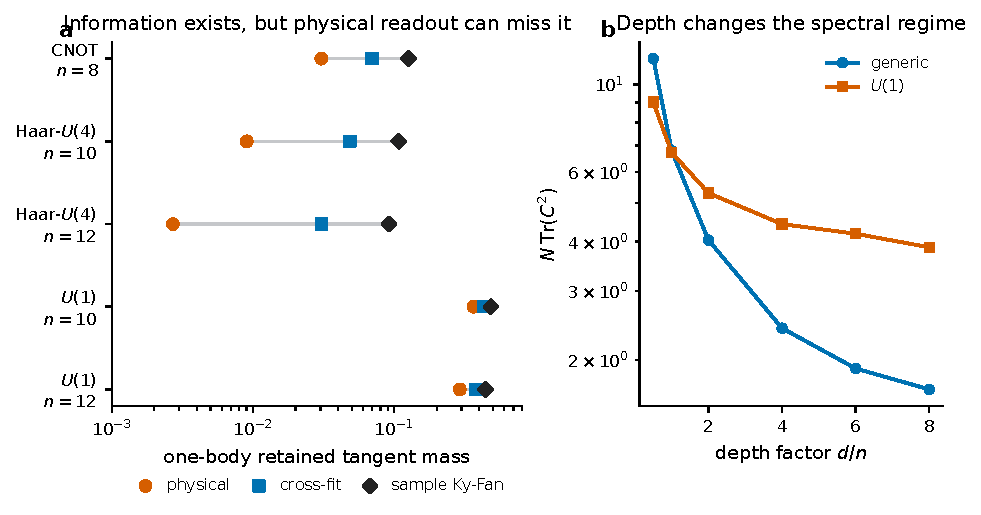
\includegraphics[width=\textwidth]{fig4_spectral_mechanism_depth.pdf}
\caption{Spectral comparison. (a) Representative one-body cells from the dedicated $M=512$ profile. In the generic Haar-$U(4)$ cells, rank-matched leading subspaces retain much more tangent mass than the physical one-body readout. The $U(1)$ readout is closer to the spectral benchmarks. (b) At $n=8$, increasing depth lowers the normalized covariance purity more rapidly for the generic circuits than for the $U(1)$ circuit.}
\label{fig:spectrum}
\end{figure*}

\section{Full-record Fisher information}

The complete computational-basis record retains an order-one fraction of QFI in both sets of circuits. In the family-balanced generic data, $F_{\rm full}/F_Q$ is about $0.488$ at $n=6$, $0.495$ at $n=16$, and $0.497$ in the targeted Haar-$U(4)$ $n=18$ test. The $U(1)$ values remain near $0.47$--$0.48$. The difference at the full-record level is modest compared with the difference after one-body projection.

Figure~\ref{fig:fullrecord} shows these quantities on the same scale. The large separation in low-weight retention appears after restricting the measured score to the small observable subspace.

\begin{figure*}[t]

\includegraphics[width=\textwidth]{fig5_full_record_vs_accessible.pdf}
\caption{Full-record and low-weight information. (a) The complete computational-basis record retains a similar order-one fraction of QFI in the generic/Haar and $U(1)$ circuits. (b) Their one-body retained fractions differ by orders of magnitude at large $n$. (c) Selected sizes plotted against $F_{\rm full}/F_Q$ show that similar full-record Fisher fractions can correspond to very different low-weight accessibility.}
\label{fig:fullrecord}
\end{figure*}

\section{Relation to quantum machine learning}

State-space geometry and measurement-accessible geometry answer different questions. QFI and the quantum geometric tensor characterize sensitivity before a measurement is selected \cite{BraunsteinCaves1994,Stokes2020,Haug2021}. Once a measurement and feature span are fixed, the accessible geometry depends on those choices \cite{HottaOzawa2004,LuLuoOh2012}. Whether the accessible directions help a learning task additionally depends on the data encoding, labels, loss function, and optimization trajectory \cite{SchuldKilloran2019,Havlicek2019,Thanasilp2023}.

For fixed Pauli weight, Eq.~\eqref{eq:fixed-weight} gives a random-orientation retained fraction of order $\mathrm{poly}(n)/2^n$. This is a statement about measurement-accessible tangent mass, not about $\mathrm{Var}(\partial_\theta L)$. It is nevertheless relevant to the trainability literature because cost locality and observable structure can change gradient scaling \cite{Cerezo2021,UvarovBiamonte2021,HolmesSharma2022}. A direct barren-plateau test can therefore record full tangent sensitivity, observable-accessible sensitivity, and task-gradient variance on the same circuit instances.

The spectral calculation also gives an ansatz--measurement design criterion. Two readout subspaces with the same rank can retain very different tangent mass. In that setting, increasing the number of observables and changing which observables are measured are different interventions. Existing work has already shown that measurement strategy can be used to diagnose or avoid unfavorable trainability regions in other settings \cite{Sack2022}. The quantities used here give a direct way to check whether a physically simple feature span intersects the leading tangent modes before a full training experiment is run.

The $U(1)$ data add a symmetry-specific observation. Symmetry-preserving and equivariant circuit constructions are used in variational algorithms and QML to restrict the model to relevant sectors or encode known invariances \cite{Gard2020,LaroccaInvariant2022,Meyer2023}. Our result is more limited: in this circuit family, the symmetry-constrained tangent covariance is concentrated and its leading structure is unusually visible to low-weight diagonal observables. This does not imply that symmetry alone improves a learning task. Accessibility and task discriminativeness remain separate questions.

\section{Scope and limitations}

The main numerical statements use a frozen protocol, circuit-level bootstrap resampling, equal weighting of the generic families, and a prespecified equivalence band. Family-level failures were retained. Leave-one-family-out sensitivity checks show that the primary generic point estimates are not set by one architecture.

The campaign includes separate basis, direction-sampler, coordinate-visibility, tangent-count convergence, depth, orientation, and spectrum profiles. The basis and direction-sampler effects are generally small in absolute size but are not zero. The coordinate sampler probes a different visibility endpoint from the dense Gaussian tangent covariance. In the nested $M=32,64,128,256$ study, a small number of cells miss the strict preregistered convergence threshold; those misses limit precision claims for the affected cells.

The asymptotic theorem is a theorem for random relative orientation. It does not prove that any physical family converges to that ensemble. The $n=18$ nonconserving stress test contains only Haar-$U(4)$. The larger-size profiles use fewer tangent directions than the primary profile. All simulations are noiseless and use diagonal low-weight $Z$ readout. Noise can change trainability and measurement statistics in variational circuits \cite{Wang2021}, and other POVMs or finite-shot estimators can change the accessible score geometry. These cases are outside the present numerical study.

A direct follow-up for QML would measure loss-gradient variance together with full and accessible tangent sensitivity on the same circuits. That experiment would test whether the accessibility quantities introduced here predict task-level gradient concentration.

\section{Discussion}

The data support a simple separation. The readout rank sets a useful reference value because a random rank-$r$ subspace has mean overlap $r/N$ with any trace-one covariance. The covariance spectrum controls the width of that random-orientation overlap. A physical circuit can still have a systematic positive or negative orientation bias.

This separation explains the generic finite-size data. The covariance becomes strongly anisotropic with $n$, while the family-balanced low-weight overlap remains inside the practical rank-equivalence band. The two observations concern different properties of $C$ and $P$. The RY--RZ--CZ family then provides a negative orientation bias within the same protocol, and the $U(1)$ family provides a much larger positive bias. The full-record Fisher calculation shows that these low-weight differences are not accompanied by a comparable separation in $F_{\rm full}/F_Q$.

The spectral profile is useful because it distinguishes missing information from inaccessible information at fixed rank. In the generic Haar-$U(4)$ example, the leading rank-matched subspace contains substantially more tangent mass than the physical one-body span. For the $U(1)$ example, the physical span is closer to the leading spectral subspace. This comparison motivates observable co-design. The relevant diagnostic is the tangent mass captured by the readout, in addition to the readout rank.

\section{Conclusion}

We studied the covariance of normalized measurement scores induced by quantum-state tangents and asked how much of that covariance is visible to a fixed low-weight readout. For random relative orientation, the rank-normalized overlap has mean one and variance bounded by $2/(r\deff)$. The result allows strong anisotropy and gives a fixed-weight retained fraction of order $n^k/2^n$ under the random-orientation model.

In the finite-size data, the family-balanced nonconserving circuits are practically rank typical while their covariance becomes increasingly anisotropic. RY--RZ--CZ has a persistent one-body deficit, whereas the half-filled $U(1)$ circuit has much larger low-weight retention and a smaller gap between the physical readout and rank-matched leading tangent subspaces. Readout rank is therefore useful as a reference value; the architecture-dependent correction is encoded in spectral orientation.

\begin{acknowledgments}
The author thanks Mohamed Bennai (\href{https://orcid.org/0000-0002-7364-5171}{ORCID: 0000-0002-7364-5171}) for helpful discussions. ChatGPT (OpenAI) was used for language editing and revision of the manuscript. The author reviewed the scientific content and approved the final text.
\end{acknowledgments}

\section*{Data and code availability}
The frozen protocols, source code, aggregate tables, and shard-level numerical outputs used in this manuscript are available in the \href{https://github.com/AHDMarwan/Spectral-Geometry-of-Accessible-Quantum-Tangents-Beyond-Isotropic-Readout-Rank-Laws}{public project repository}. The principal result archives are \texttt{rigorous-v2\_primary}, \texttt{rigorous-v2\_large\_n}, and \texttt{rigorous-v2\_n18}. The asymptotic derivation is included with the paper sources.

\appendix

\section{Random-projector second moment}\label{app:random-projector}
Let $P$ be the orthogonal projector onto a Haar-uniform real rank-$r$ subspace of $\mathbb{R}^N$. Orthogonal invariance and standard Grassmann/Haar integration formulas \cite{CollinsMatsumoto2017,Bendokat2024} give
\begin{equation}
\mathbb{E}[P_{ij}P_{kl}]=a\,\delta_{ij}\delta_{kl}+b(\delta_{ik}\delta_{jl}+\delta_{il}\delta_{jk}).
\end{equation}
The identities $\Tr P=r$ and $\Tr P^2=r$ imply
\begin{align}
aN^2+2bN&=r^2,\\
aN+b(N^2+N)&=r,
\end{align}
so
\begin{align}
a&=\frac{r(Nr+r-2)}{N(N-1)(N+2)},\\
b&=\frac{r(N-r)}{N(N-1)(N+2)}.
\end{align}
For a fixed real symmetric $C$ with $\Tr C=1$,
\begin{equation}
\mathbb{E}\!\left[\Tr(PC)^2\right]=a+2b\Tr(C^2).
\end{equation}
Subtracting $(r/N)^2$ gives
\begin{equation}
\mathrm{Var}[\Tr(PC)]=\frac{2r(N-r)\left[N\Tr(C^2)-1\right]}{N^2(N-1)(N+2)}.
\end{equation}
For $\rho=\Tr(PC)/(r/N)$,
\begin{equation}
\mathrm{Var}(\rho)=\frac{2(N-r)\left[N\Tr(C^2)-1\right]}{r(N-1)(N+2)}.
\end{equation}
Writing $q=\Tr(C^2)$ and using $N-r\le N-1$ and $Nq-1\le q(N+2)$ gives
\begin{equation}
\mathrm{Var}(\rho)\le\frac{2q}{r}=\frac{2}{r\deff}.
\end{equation}
Figure~\ref{fig:nullwidth} compares the exact standard deviation with the simpler envelope.

\begin{figure}[t]
\centering
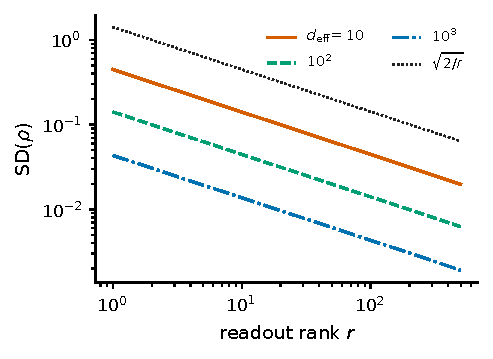
\includegraphics[width=.49\linewidth]{figS2_exact_null_width.pdf}
\caption{Exact random-orientation standard deviation at $N=2^{14}-1$ for representative $\deff$, together with the covariance-independent $\sqrt{2/r}$ envelope.}
\label{fig:nullwidth}
\end{figure}

\section{Effective spectral fraction}\label{app:deff-fraction}
Figure~\ref{fig:defffrac} plots $\deff/N$. It decreases with system size for both circuit groups over the tested range.
\begin{figure}[t]
\centering

\includegraphics[width=.49\linewidth]{figS1_deff_fraction.pdf}
\caption{Effective dimension as a fraction of score-space dimension. The nonconserving $n=18$ point is the targeted Haar-$U(4)$ stress test.}
\label{fig:defffrac}
\end{figure}

\section{Orientation diagnostic}\label{app:orientation-diagnostic}
The main text emphasizes raw retention and $\rho$. The post-hoc population-null $z$ statistic is algebraically tied to $\rho-1$, so it is not treated as independent evidence. Figure~\ref{fig:zdiag} reports the large-size values for completeness.
\begin{figure}[t]
\centering

\includegraphics[width=.49\linewidth]{figS3_orientation_z.pdf}
\caption{Population-null orientation diagnostic for selected large-$n$ cells. The vertical axis uses a symmetric logarithmic scale.}
\label{fig:zdiag}
\end{figure}

\section{Rank fraction for fixed Pauli weight}\label{app:rank-fraction}
For full computational-basis support, the centered score-space dimension is exponential in $n$ while the number of diagonal Pauli-$Z$ strings through fixed weight is polynomial. Figure~\ref{fig:rankfrac} shows the corresponding rank fractions.
\begin{figure}[t]
\centering
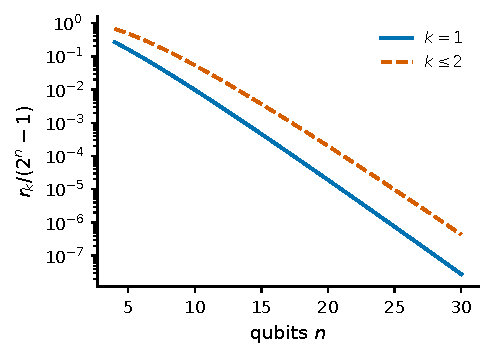
\includegraphics[width=.52\linewidth]{figS4_rank_fraction.pdf}
\caption{Full-support rank fraction for one-body and up-to-two-body diagonal Pauli-$Z$ readouts. This full-support formula is not used for the symmetry-reduced $U(1)$ sector; there the archived score dimension and measured readout rank are used.}
\label{fig:rankfrac}
\end{figure}

\section{Status of the numerical claims}\label{app:evidence-status}
\begin{table*}[t]
\caption{Evidence status for the main numerical statements. ``Confirmatory'' refers to quantities and decision rules fixed before the corresponding rigorous-v2 outcomes were inspected.}
\centering
\begin{tabular}{@{}ll@{}}
\toprule
\parbox[t]{0.25\textwidth}{\textbf{Claim}} & \parbox[t]{0.68\textwidth}{\textbf{Evidence status}} \\
\midrule
\parbox[t]{0.25\textwidth}{Generic practical rank typicality} & \parbox[t]{0.68\textwidth}{Confirmatory family-balanced primary inference for $n=6$--$12$, prespecified large-$n$ extension for $n=14,16$, and targeted Haar-$U(4)$ stress test at $n=18$.} \\
\parbox[t]{0.25\textwidth}{Rank typicality with anisotropic covariance} & \parbox[t]{0.68\textwidth}{Exact random-orientation theorem plus confirmatory coexistence of $\rho\simeq1$ with increasing $N\Tr(C^2)$.} \\
\parbox[t]{0.25\textwidth}{RY--RZ--CZ one-body deficit} & \parbox[t]{0.68\textwidth}{Confirmatory family-resolved exception; entire confidence intervals lie below $0.90$ at $n=14,16$.} \\
\parbox[t]{0.25\textwidth}{$U(1)$ low-weight alignment} & \parbox[t]{0.68\textwidth}{Prespecified finite-size enhancement and orientation contrasts through $n=18$; no asymptotic enhancement exponent is claimed.} \\
\parbox[t]{0.25\textwidth}{Generic information present at the same rank} & \parbox[t]{0.68\textwidth}{Dedicated $M=512$ spectral profile comparing physical, cross-fit, and same-sample Ky Fan retention.} \\
\parbox[t]{0.25\textwidth}{Population-null bridge scaling} & \parbox[t]{0.68\textwidth}{Exploratory post-hoc reanalysis of archived circuits; no new quantum simulations and no primary confirmatory status.} \\
\bottomrule
\end{tabular}
\end{table*}

\begin{thebibliography}{99}

\bibitem{BraunsteinCaves1994}
S. L. Braunstein and C. M. Caves,
Statistical distance and the geometry of quantum states,
Phys. Rev. Lett. \textbf{72}, 3439 (1994),
doi:10.1103/PhysRevLett.72.3439.

\bibitem{HottaOzawa2004}
M. Hotta and M. Ozawa,
Quantum estimation by local observables,
Phys. Rev. A \textbf{70}, 022327 (2004),
doi:10.1103/PhysRevA.70.022327.

\bibitem{LuLuoOh2012}
X.-M. Lu, S. Luo, and C. H. Oh,
Hierarchy of measurement-induced Fisher information for composite states,
Phys. Rev. A \textbf{86}, 022342 (2012),
doi:10.1103/PhysRevA.86.022342.

\bibitem{Stokes2020}
J. Stokes, J. Izaac, N. Killoran, and G. Carleo,
Quantum Natural Gradient,
Quantum \textbf{4}, 269 (2020),
doi:10.22331/q-2020-05-25-269.

\bibitem{Haug2021}
T. Haug, K. Bharti, and M. S. Kim,
Capacity and Quantum Geometry of Parametrized Quantum Circuits,
PRX Quantum \textbf{2}, 040309 (2021),
doi:10.1103/PRXQuantum.2.040309.

\bibitem{Sim2019}
S. Sim, P. D. Johnson, and A. Aspuru-Guzik,
Expressibility and Entangling Capability of Parameterized Quantum Circuits for Hybrid Quantum-Classical Algorithms,
Adv. Quantum Technol. \textbf{2}, 1900070 (2019),
doi:10.1002/qute.201900070.

\bibitem{McClean2018}
J. R. McClean, S. Boixo, V. N. Smelyanskiy, R. Babbush, and H. Neven,
Barren plateaus in quantum neural network training landscapes,
Nat. Commun. \textbf{9}, 4812 (2018),
doi:10.1038/s41467-018-07090-4.

\bibitem{Cerezo2021}
M. Cerezo, A. Sone, T. Volkoff, L. Cincio, and P. J. Coles,
Cost function dependent barren plateaus in shallow parametrized quantum circuits,
Nat. Commun. \textbf{12}, 1791 (2021),
doi:10.1038/s41467-021-21728-w.

\bibitem{UvarovBiamonte2021}
A. Uvarov and J. Biamonte,
On barren plateaus and cost function locality in variational quantum algorithms,
J. Phys. A: Math. Theor. \textbf{54}, 245301 (2021),
doi:10.1088/1751-8121/abfac7.

\bibitem{HolmesSharma2022}
Z. Holmes, K. Sharma, M. Cerezo, and P. J. Coles,
Connecting Ansatz Expressibility to Gradient Magnitudes and Barren Plateaus,
PRX Quantum \textbf{3}, 010313 (2022),
doi:10.1103/PRXQuantum.3.010313.

\bibitem{Larocca2022}
M. Larocca, P. Czarnik, K. Sharma, G. Muraleedharan, P. J. Coles, and M. Cerezo,
Diagnosing Barren Plateaus with Tools from Quantum Optimal Control,
Quantum \textbf{6}, 824 (2022),
doi:10.22331/q-2022-09-29-824.

\bibitem{Pesah2021}
A. Pesah, M. Cerezo, S. Wang, T. Volkoff, A. T. Sornborger, and P. J. Coles,
Absence of Barren Plateaus in Quantum Convolutional Neural Networks,
Phys. Rev. X \textbf{11}, 041011 (2021),
doi:10.1103/PhysRevX.11.041011.

\bibitem{Wang2021}
S. Wang, E. Fontana, M. Cerezo, K. Sharma, A. Sone, L. Cincio, and P. J. Coles,
Noise-induced barren plateaus in variational quantum algorithms,
Nat. Commun. \textbf{12}, 6961 (2021),
doi:10.1038/s41467-021-27045-6.

\bibitem{Thanasilp2023}
S. Thanasilp, S. Wang, N. A. Nghiem, P. J. Coles, and M. Cerezo,
Subtleties in the trainability of quantum machine learning models,
Quantum Mach. Intell. \textbf{5}, 21 (2023),
doi:10.1007/s42484-023-00103-6.

\bibitem{Sack2022}
S. H. Sack, R. A. Medina, A. A. Michailidis, R. Kueng, and M. Serbyn,
Avoiding Barren Plateaus Using Classical Shadows,
PRX Quantum \textbf{3}, 020365 (2022),
doi:10.1103/PRXQuantum.3.020365.

\bibitem{Gard2020}
B. T. Gard, L. Zhu, G. S. Barron, N. J. Mayhall, S. E. Economou, and E. Barnes,
Efficient symmetry-preserving state preparation circuits for the variational quantum eigensolver algorithm,
npj Quantum Inf. \textbf{6}, 10 (2020),
doi:10.1038/s41534-019-0240-1.

\bibitem{LaroccaInvariant2022}
M. Larocca, F. Sauvage, F. M. Sbahi, G. Verdon, P. J. Coles, and M. Cerezo,
Group-Invariant Quantum Machine Learning,
PRX Quantum \textbf{3}, 030341 (2022),
doi:10.1103/PRXQuantum.3.030341.

\bibitem{Meyer2023}
J. J. Meyer, M. Mularski, E. Gil-Fuster, A. A. Mele, F. Arzani, A. Wilms, and J. Eisert,
Exploiting Symmetry in Variational Quantum Machine Learning,
PRX Quantum \textbf{4}, 010328 (2023),
doi:10.1103/PRXQuantum.4.010328.

\bibitem{KyFan1949}
K. Fan,
On a Theorem of Weyl Concerning Eigenvalues of Linear Transformations I,
Proc. Natl. Acad. Sci. USA \textbf{35}, 652 (1949),
doi:10.1073/pnas.35.11.652.

\bibitem{CollinsMatsumoto2017}
B. Collins and S. Matsumoto,
Weingarten calculus via orthogonality relations: new applications,
ALEA Lat. Am. J. Probab. Math. Stat. \textbf{14}, 631 (2017),
doi:10.30757/ALEA.v14-31.

\bibitem{Bendokat2024}
T. Bendokat, R. Zimmermann, and P.-A. Absil,
A Grassmann Manifold Handbook: Basic Geometry and Computational Aspects,
Adv. Comput. Math. \textbf{50}, 6 (2024),
doi:10.1007/s10444-023-10090-8.


\bibitem{SchuldKilloran2019}
M. Schuld and N. Killoran,
Quantum Machine Learning in Feature Hilbert Spaces,
Phys. Rev. Lett. \textbf{122}, 040504 (2019),
doi:10.1103/PhysRevLett.122.040504.

\bibitem{Havlicek2019}
V. Havl\'{i}\v{c}ek, A. D. C\'{o}rcoles, K. Temme, A. W. Harrow, A. Kandala, J. M. Chow, and J. M. Gambetta,
Supervised learning with quantum-enhanced feature spaces,
Nature \textbf{567}, 209 (2019),
doi:10.1038/s41586-019-0980-2.

\bibitem{Efron1979}
B. Efron,
Bootstrap Methods: Another Look at the Jackknife,
Ann. Stat. \textbf{7}, 1 (1979),
doi:10.1214/aos/1176344552.

\end{thebibliography}


\end{document}
